\documentclass[twocolumn,9pt]{jsproceedings}
\RequirePackage[l2tabu,orthodox]{nag}  % 古いコマンドやパッケージを使用した場合に警告する
\usepackage[all,warning]{onlyamsmath}  % amsmath が提供しない数式環境を使用した場合に警告する
% \usepackage{flushend}  % 最終ページの2カラムの左右の高さを揃える
\usepackage{here} %図の場所の指定で[h](ここに貼る)を指定するためのパッケージ
\usepackage[dvipdfmx]{graphicx} %dvipdfmxはjpgやpngの張り込みのために使用


% タイトル
\title{2D LiDARを搭載した小型移動ロボットでの\\つくばチャレンジ2022参加レポート}

\author{○池邉 龍宏\authorrefmark{1}, 内田 璃空\authorrefmark{1}, 畑中 優一郎\authorrefmark{1}, 林原 靖男\authorrefmark{1}, 上田 隆一\authorrefmark{1}}

\etitle{Participation report in the Tsukuba Challenge 2022\\using a small mobile robot with 2D LiDAR}

\eauthor{○Tatsuhiro IKEBE\eauthorrefmark{1}, Riku UCHIDA\eauthorrefmark{1}, Yuichiro HATANAKA\eauthorrefmark{1}, \\Yasuo HAYASHIBARA\eauthorrefmark{1}, Ryuichi UEDA\eauthorrefmark{1}}

\affiliation{千葉工業大学 未来ロボティクス学科 Cat Aチーム}

% \abstract{
% }

% \keywords{}

\begin{document}
\maketitle

\authorreftext{1}{千葉工業大学先進工学部未来ロボティクス学科}
\authorreftext{2}{千葉工業大学先進工学研究科未来ロボティクス専攻}
\eauthorreftext{1}{Department of Advanced Robotics, Faculty of Advanced Engineering, Chiba Institute of Technology}
\eauthorreftext{2}{Department of Advanced Robotics, Graduate School of Advanced Engineering, Chiba Institute of Technology}

%句読点はあとからsedで統一しましょう

% 本文
\section{緒言}

千葉工業大学未来ロボティクス学科Cat Aチーム/Bチームは,
図\ref{fig:raspicat}に見られる小型で簡素なセンサ構成のロボットを,
屋外で安定して自律走行させるためのソフトウェアを研究している.
簡素さをテーマにするのは,
安価な屋外移動ロボットのシステムの実現と,
情報が不確かなときのロボットの巧妙な振る舞いの研究に興味があるからである.
最新,高性能のセンサを次々に導入する方針だと,
アルゴリズムの工夫にかける時間や動機が減り,
また,ロボットの計算機,台車,電池の大型化,
製作,メンテナンス費用の増大を招く.
そこで,あえて計算負荷の低いセンサと
小型の計算機での安定した自己位置推定やナビゲーション
の実現に取り組んでいる.


本年度は,
\begin{itemize}
\item 計算機としてRaspberry Pi4のみを使用
\item 外界センサとして2次元LiDARのみを使用
\item 移動量の算出に内界センサ(IMUやオドメータ)を不使用
\end{itemize}
という構成で,つくばチャレンジ本走行での完走を試みた.
昨年度はノート型PCを計算機として使用したが,
本年度は用いず,ナビゲーションに関する全ての計算を
Raspberry Pi4ひとつで実現した.


\begin{figure}[h]
 	\begin{center}
 		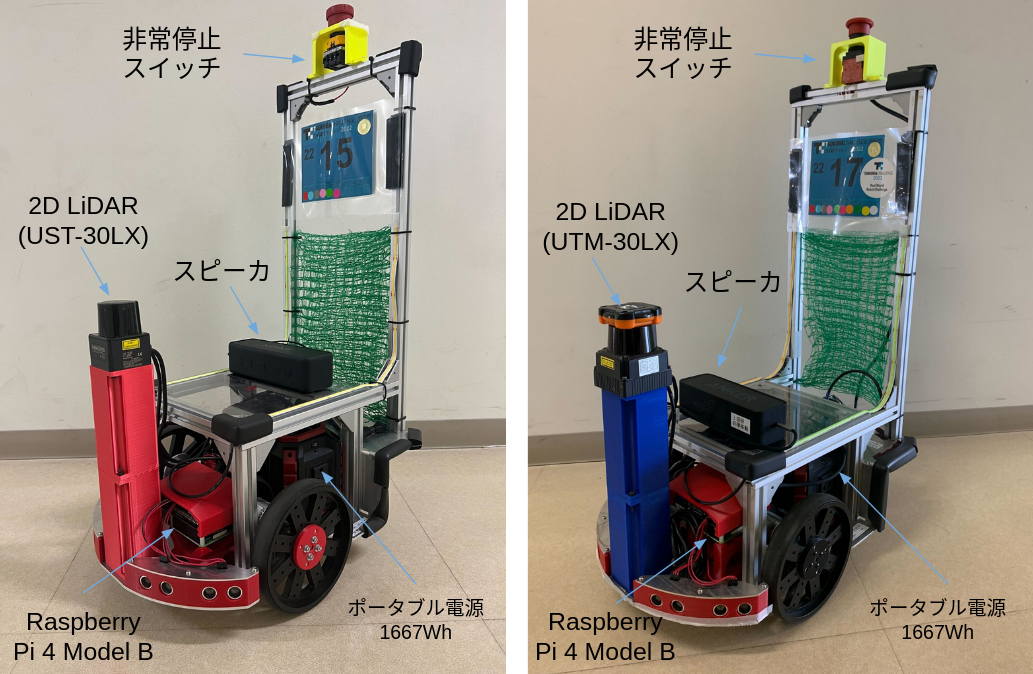
\includegraphics[width=1.0\linewidth]{figs/raspicat.png}
 		\caption{Raspberry Pi Cat(つくばチャレンジ2022)}
 		\label{fig:raspicat}
 	\end{center}
\end{figure}

本年度の本走行の結果をTable \ref{MainRun}に示す.
記録としては確認走行区間の終わりか,少し超えた程度の
地点までしか到達できなかったが,
Bチームは,ノートPCを計算機に用いた昨年の成績を上回った.
また,実験走行では4回の人の介入のみでゴールまで到達することができ,
完走に向けて目処が立った.

\begin{table}[h]
  \caption{各チームの本走行の結果}
  \label{MainRun}
	\begin{tabular}{|c|c|p{5.4cm}|}
    \hline
	チーム & 走行距離 & リタイアの理由 \\
    \hline
	A & 200[m] & 市役所前の横断歩道の横断直前で,点字ブロックに車輪を取られ自己位置を見失った.\\
    \hline
	B & 369[m] & 2つめの一時停止地点において一時停止の規則に違反した. \\ 
    \hline
  \end{tabular}
\end{table}


本稿では,本チームのような2次元LiDAR,Raspberry Pi
という構成での移動ロボットの構築方法を説明する.
また,この構成で特に重要となる自己位置推定について,
つくばチャレンジで起こったことを踏まえて議論する.
本稿の構成は次の通りである. 
2章, 3章では, 参加したロボットの構成について, 
それぞれハードウェア, ソフトウェアの面から説明する. 
4章では本年度のつくばチャレンジでのチームの活動や, 
実験走行, 本走行での結果を説明する.
5章で考察を行い, 6章で得られた知見, 7章で結言を述べる. 
@@@変更あり@@@

\section{実験結果}

各チームの走行結果を表\ref{table:MainRun}にまとめた.
どちらのチームも自己位置が破綻し,リタイアとなった.


なお,Cat Aチームは実験走行で,4回人の手を加えつつもスタートからゴールまで走行できた.
表\ref{table:4hands}に手を加えた箇所をまとめた.

\begin{table}[h]
  \label{4hands}
  \begin{tabular}{|l|l|}
    \hline
    手を加えたポイント & 原因 \\
    \hline
    信号有り横断歩道西側の歩道 & コーンとの衝突 \\
    \hline
    信号有り横断歩道の横断中 & 対向ロボットとの衝突 \\ 
    \hline
    公園エリアの横断歩道の手前 & コーンとの衝突 \\ 
    \hline
    信号有り横断歩道西側の歩道 & 自己位置の喪失 \\ 
    \hline
  \end{tabular}
  \caption{人の手を加えた箇所}
\end{table}

障害物回避ができなかったため人の手が加わることが多くあった.

\section{自己位置推定}

\subsection{自己位置推定のシステム}

自己位置推定に関連するシステムを
図\ref{fig:ハードウェア}, 図\ref{fig:ソフトウェア}に示す. 
自己位置推定に使用した外界センサは, 2D LiDARのみであり,
この2D LiDARを去年\cite{去年のつくばチャレンジシンポジウム}
と同様に同じ位置に取り付けた.
IMUなどの慣性計測装置は, 去年で使用せずに550m自律走行することができたことから, 
つくばチャレンジ2022で使用しなかった. 

ロボットの制御システムとしてROSを使用している. 
経路計画, 経路追従, 障害物回避は, ROSがOSSとして公開している
NavigationStackを使用した. 
自己位置推定は, 去年amclを使用していたが, 
今年は, 当チームの研究室の教員である上田 隆一が開発したemcl2を使用した. 

\subsection{見つかった問題}

今回実験走行/本走行で自己位置推定を行うことが難しい環境に遭遇した. 
難しかった環境は, 図\ref{fig:自己位置推定難しかったマップ}で示された
\begin{itemize}
  \item 信号あり横断歩道の停止線前の20m
  \item 信号あり横断歩道行き(2回目の停止線での停止)
  \item 信号あり横断歩道行き(横断歩道の横断)
  \item 市役所側の線路隣の路地
  \item 公園側の線路隣の路地
\end{itemize}
である. 

信号あり横断歩道の停止線前の20m, 市役所側の線路隣の路地, 公園側の線路隣の路地は, 
ロボットが移動しているが自己位置推定側のパーティクルが移動しない問題があった. 
信号あり横断歩道行き全般(2回目の停止線での停止)は, 停止エリアに点字ブロックが存在し,
また2D LiDAR前方のほとんどのセンサ情報が地面になってしまうほどの勾配になっており, 自己位置推定が不確かであった.
信号あり横断歩道行き(横断歩道の横断)は, 点字ブロックに足を大きく持っていかれ回転方向に大きく自己位置推定が
ずれたり, ランドーマークを観測できてない状況での膨張リセットが働いたため自己位置推定の破綻を起こすことがあった. 


%\section{実験走行,本走行の結果}←ここにもってくる

% \section{ハードウェア}

% つくばチャレンジ2022で使用したロボットは, 
% 既製品のRaspberry Pi Cat(以下ラズパイキャットと呼ぶ)\cite{RTshop}である.
% 図\ref{fig:raspicat}に使用した機体を示す.
% 本章では,このロボットについて去年との差分を含めて説明をする.


% \subsection{ハードウェア構成}

% %まず,何が特徴なのか,なにが狙いなのかを説明してから全体の話をする.(ちゃんとできるようになって!!)

% Aチーム,Bチームとも,機体として既成品のRaspberry Pi Catを購入した.Raspberry Pi CatはモータのコントローラとしてRaspberry Piが使用されている.今年度は,このRaspberry Piで自己位置推定やナビゲーションのソフトウェアを実行することで,Raspberry Piのみを計算資源としたナビゲーションに挑戦した.

% Aチームの機体に搭載されている, 計算機,センサ,アクチュエータは図\ref{fig:raspicat}のように接続されている.
% 機体の主な計算機として, ラズパイ4を搭載しており, 外界センサとして
% 2D LiDAR(UST 30LX)を使用している.2D LiDARは,ラズパイ4とehernetケーブルで接続されている.
% アクチュエータとしては,DCモータを使用している. DCモータはラズパイの上に乗っているDCモータドライバ
% と接続されている.電源としては,12V出力のモバイルバッテリを搭載しており,ラズパイ4やDCモータドライバに電力を供給する.

% 機体の速度指令値はラズパイ4で計算し, デバイスドライバによってPWMに変換され,DCモータドライバに入力される.
% 自己位置推定や障害物回避は,速度指令値を積算させたデッドレコニングと2D LiDARのみで行っている.

% \subsection{去年との差分} %これ,まとめて書かないで,各議論のときに触れるとよいです.(そうしないとなんのために説明しているのか分からない)
 
% 去年使用した機体を図\ref{fig:raspicat}に示す. 
% 去年の機体と比較して機体のサイズに関わる部分に関して変更はない.
% 主な差分としては, 自律移動を行うために使用する計算機として
% ゲーミングPCからラズパイに変更, ギア比の高いモータへ変更, スピーカを搭載
% が挙げられる.

% %↓3年生書いて.Aチームと統一感のある写真も提供を.
% Bチームでは,@@@はAチームと共通であるが,@@@が異なる.


% %↓ここらへんの細かい話は,上で概要が説明してあれば,あとから議論,評価するときでいいと思います.

% \subsection{計算機の変更}

% 今年は, ラズパイ4のみで自律移動を行った.%これは目玉というか他チームとの違いとしてもっと早い段階でいうべきこと.(ということで上に書きました)
% これは, ここでも話されていたラズパイのみで自律移動を行うという試みを
% 今年のつくばチャレンジ2022で試みたものである.

% \subsection{ギア比の高いモータへ変更}

% 去年使用した機体はraspicatで今年使用した機体はraspicatであり,V2になってからモータのギヤ比が高くなった.
% これにより,〜が向上し(書く必要ある?)%何かを説明するときに必要になったら書くことで,主なこととして書くことではないと思います.

% \subsection{スピーカを搭載}

% ラズパイ4のみで自律移動を行っているためリアルタイムでの処理のデバッグを行うのが困難であった.
% そのため,スピーカを搭載し,ある処理を行った場合にある特定の日本語を喋らせることで, 
% 音声によるデバッグを行えるようにした.%便利だったとアピールしましょう.(ソフトウェアパッケージになっているなら宣伝を)

% \subsection{2D LiDARの取り付け位置}

% %↓「高い位置に取り付けることで,xxxxを防いだ」とか,主文で意図まで踏み込んで書かないと,「ふーん.で?」になっちゃうので,メモ書きでもそこは意識すること.
% 当チームの機体の2D LiDARは, 他のチームの機体と比べて高い位置に取り付けられている.
% \cite{RTshop}
% これによりxxxxだったものがyyyy向上した.

% \subsection{ジャイロ, IMU, ロータリーエンコーダ不使用の判断}

% %ここは詳しく書きたいところです.(重要な順に書くものなので,たぶんLiDARの取り付け位置より上?)

% \section{ソフトウェア}

% 本章では,ソフトウェア構成の他,
% 安定した自律走行をさせるために工夫したことなどについて説明する.


% \subsection{ソフトウェアの構成}

% \subsection{GIMPによるマップの合成} %他のチームでもやっていることなら省く

% \subsection{経路計画のためのマップ編集}


% \subsection{自己位置推定テストR}

% \subsection{シミュレーション環境でのナビゲーションのテスト}

% %上に持っていく\section{つくばチャレンジ2022での走行結果}
% (cat aチームの話は内田くんがあとから追記する)
% \subsection{自己位置推定の調整(10月9日,10月23日, 11月7日)}


% \subsection{試走と本走行(11月19日〜本走行)}


\section{考察}

\subsection{環境の段差と小型ロボット}

当チームのロボットは他のチームと比較して小型のロボットである.
車輪径は30cmであり,なんとか道路と横断歩道の段差を乗り越えることができている.
つくばチャレンジ2022の走行結果に書かれている通り,点字ブロックにおいては対応ができていない.
信号あり横断歩道を渡る前の停止線では点字ブロックが原因で渡る前に足を持っていかれたり,
停止線する時に足を持っていかれることでうまく停止できないことがあった.
これは,小型ロボットゆえでもあり,当チームの自己位置推定が期待通りに機能できてないといえる.

\subsection{2DLiDARのみでの自己位置推定}

つくばチャレンジ2021では,当チームは2DLiDARのみによる自己位置推定を行った\cite{RTshop}.
順調に信号あり横断歩道まで走行ができたため,つくばチャレンジ2022では同じセンサ構成で挑んだ.

つくばチャレンジ2022では,つくばチャレンジ2021で走行できなかった
信号あり横断歩道から→研究学園駅→公園→ゴールまでの箇所のナビゲーションを行った.
人混みや信号あり横断歩道の停止線での待機列に遭遇しない,点字ブロックに大きく足を持っていかれない場合において
順調に自己位置推定を行うことができた.
人混みや待機列に遭遇した場合は2D LiDARほぼすべてのデータが未知障害物であり,地図との照合に使用できない.
点字ブロックにおいては

\section{知見}


\section{結言}

\section*{謝辞}

本実験走行の一部はJSPS科研費JP20K04382の助成を受けました.また,つくばチャレンジ実行委員会,つくば市の皆様に感謝申し上げます.

%↑上田整理.あと,著者に名前を連ねない人がいたらここに書くと良いです.

% 参考文献
% \small
\footnotesize
\begin{thebibliography}{99}
  \bibitem{ROS}
	  Morgan Quigley {\it et al.}: ``ROS: an open-source Robot Operating System,'' 
Open-Source Software workshop of the International Conference on Robotics and Automation, 2009. 

\bibitem{ueda2002tdp}
	Ryuichi Ueda {\it et al.}: 
``Team description of Team ARAIBO,'' 
Proc. of 2002 International RoboCup Symposium, 2002. 

  \bibitem{ueda2004iros}
	Ryuichi Ueda {\it et al.}: 
  ``Expansion Resetting for Recovery from Fatal Error in Monte Carlo Localization -- Comparison with Sensor Resetting Methods,'' Proc.of IROS,pp.2481--2486,2004.
  
  \bibitem{map2gazebo}
  Shiloh Curtis: ``shilohc/map2gazebo'',\url{https://github.com/shilohc/map2gazebo} (last visit: 2021-12-31).
  
  \bibitem{move_base}
  Eitan Marder-Eppstein: ``move\_base,'' \url{http://wiki.ros.org/move_base} (last visit: 2021-12-31).
  
  \bibitem{amcl}
  Brian Gerkey: ``amcl,'' \url{https://wiki.ros.org/amcl} (last visit: 2021-12-31).

  \bibitem{gmapping}
  Brian Gerkey: ``gmapping,'' \url{http://wiki.ros.org/gmapping} (last visit: 2021-12-31).
  
  \bibitem{GIMP}
  GIMP.org: ``GIMP,'' \url{https://www.gimp.org/} (last visit: 2021-12-31).
  
  \bibitem{emcl}
  Ryuichi Ueda: ``ryuichiueda/emcl,''\\\url{https://github.com/ryuichiueda/emcl} (last visit: 2021-12-31).
  
  \bibitem{raspicat}
  Ryuichi Ueda and Daisuke Sato: ``ja/raspicat,'' \url{https://wiki.ros.org/ja/raspicat} (last visit: 2021-12-31).
  
  \bibitem{raspicat_rosbag}
  Tatsuhiro Ikebe: ``uhobeike/raspicat\_rosbag,'' \url{https://github.com/uhobeike/raspicat_rosbag} (last visit: 2021-12-31).


  \bibitem{池邉2021}
 池邉 龍宏,曹 越,高橋 秀太,クルス ペレス アントニオ,林原 靖男,上田 隆一: 小型移動ロボットによるつくばチャレンジへの挑戦,第22回計測自動制御学会システムインテグレーション部門講演会,pp.3390-3393,2021.

\bibitem{上田2019}
上田 隆一: ``詳解確率ロボティクス'', 講談社, 2019.

  \bibitem{上田2020}
 上田隆一,鈴木勇矢: 自己位置が不確かな状況における移動ロボットの危険回避行動の生成,第38回日本ロボット学会学術講演会予稿集,pp.RSJ2020AC2C2-02,オンライン開催,2020.

  \bibitem{地図合成}
  川合隆太他: ``産業技術大学院大学における自律移動ロボット「産技大2号」の開発'',2019年度つくばチャレンジシンポジウム, pp.4-7, 2020.

  \bibitem{RTshop}
  株式会社アールティ:``Raspberry Pi Cat 屋外でも動かせる中型2輪ロボット'',
  RT Robot Shop Products,\url{https://rt-net.jp/products/raspberry-pi-cat/} (last visit 2021-12-31)

  \bibitem{aws2020}
	  CIT自律ロボット研究室: ``AWSロボットデリバリーチャレンジで本研究室メンバーが優勝,'' \url{https://lab.ueda.tech/?post=20200915_aws_challenge} (last visit 2022-01-04)

  \bibitem{学科サイト}
	  千葉工業大学先進工学部未来ロボティクス学科: ``AWS Robot Delivery Challenge 2021 準優勝'', \url{https://www.robotics.it-chiba.ac.jp/j/?p=838} (last visit 2022-01-04)
  
  \bibitem{つくばチャレンジロボット仕様}
  つくばチャレンジ実行委員会事務局:``つくばチャレンジ 2021 ロボット仕様条件'',
  \url{https://tsukubachallenge.jp/2021/regulations/specs} (last visit 2021-12-31)
  
  \bibitem{UST-30LX}
  北陽電機株式会社:``UST-30LX'',\url{https://www.hokuyo-aut.co.jp/search/single.php?serial=195#spec} (last visit: 2021-12-31).
  
  \bibitem{Turtlebot3 Burger}
  株式会社ロボティズ: ``Turtlebot3 Burgerの仕様'',\url{https://emanual.robotis.com/docs/en/platform/turtlebot3/features/} (last visit: 2022-1-3).
  
  \bibitem{つくばチャレンジ公式記録}
  つくばチャレンジ実行委員会事務局:``つくばチャレンジ2021の走行結果'',
  \url{https://tsukubachallenge.jp/2021/records/final} (last visit 2021-12-31)

  \bibitem{出野畑中}
	  畑中 優一郎,出野 廣太郎,上田 隆一:``Raspberry Pi 3BのみでRaspberry Pi Catのナビゲーション(屋内環境編)'',CIT自律ロボット研究室,\url{https://lab.ueda.tech/?post=20211210} (last visit 2022-01-02)
\end{thebibliography}
\normalsize

\end{document}


当チームは,9日間分のすべての実験走行会に参加した.
7月2日,7月23日は確認走行区間から信号有り横断歩道手前までの自己位置推定のテストを行った.
地図は昨年作ったものを使い,自己位置推定のパッケージにemcl2を使った.
また,駅・公園エリアの地図作成のためのrosbagを取った.
9月17日,10月1日は駅・公園エリアの走行実験を行った.
走行エリアが増えたことに伴い地図の容量が増大し,4GBメモリのRaspberry Piでは処理できなかった.
メモリの容量を増やし,地図の余白部分を削ることで駅・公園エリアが走行できるようになった.
10月22日,10月23日は信号有り横断歩道の横断の走行テストを行った.
通常の走行速度では青信号中に横断しきれなかったため,
信号有り横断歩道の横断中のみ走行速度を変えることで,青信号中に横断しきることができた.
